\section{Problemstillinger ved lægemiddelskift}
Substitution af lægemidler kan medføre patientsikkerhedsmæssige konsekvenser~\citep{DanskSelskabforPatientsikkerhed2009}. Et norsk studie har undersøgt konsekvenserne ved generisk substitution~\citep{Hakonsen2010}. Interview med 100 sygeplejersker påviste at der opstod fejlmedicinering ved generiske lægemidler~\citep{Hakonsen2010}. Ud af disse følte 92~\% af sygeplejerskerne at generiske lægemidler var tidskrævende og 91~\% at risikoen for fejl øges ved disponering, hvoraf 42~\% havde oplevede fejl som følge af generisk substitution~\citep{Hakonsen2010}.
Medicineringsfejl ved generisk substitution fremgår af Figur \ref{fig:GeneriskSubstitution}.

\begin{figure}[H]\centering	\includegraphics[width=1\textwidth]{billeder/GenSub.png} 
	\caption{Medicineringsfejl ved generisk substitution rapporteret (n=100)~\citep{Hakonsen2010}.}
	\label{fig:GeneriskSubstitution}  
\end{figure}

Det fremgår af Figur \ref{fig:GeneriskSubstitution} at størstedelen af fejlmedicinering ved generisk substitution skyldes forkert lægemiddel, hvor en mindre del skyldes forkert formulering og i sjældnere tilfælde forkert dosis, administrationsvej og udeladelse af dosis. Yderligere blev årsager til fejlmedicinering rapporteret af 42 sygeplejersker~\citep{Hakonsen2010} og fremgår af Figur \ref{fig:GeneriskSubstitution1}.

\begin{figure}[H]\centering	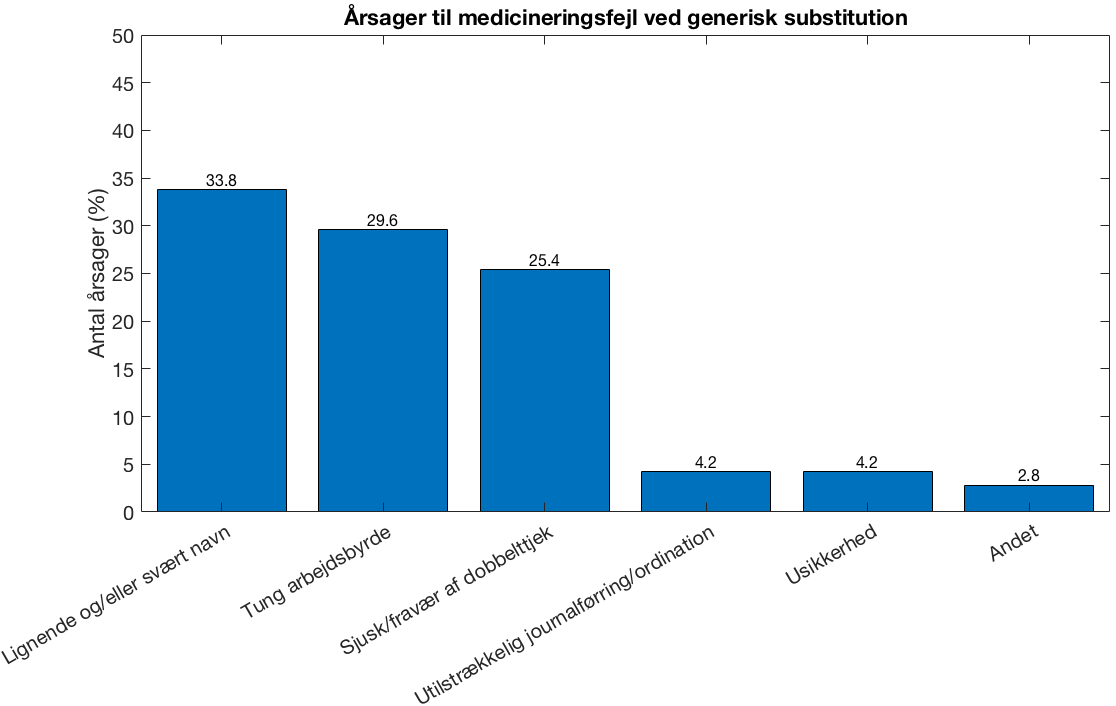
\includegraphics[width=1\textwidth]{billeder/GenSub1.png} 
	\caption{Årsager til medicineringsfejl ved generisk substitution (n=42)~\citep{Hakonsen2010}.}	\label{fig:GeneriskSubstitution1}  
\end{figure}

Af Figur \ref{fig:GeneriskSubstitution1} fremgår det at størstedelen af årsagerne til medicineringsfejl ved generisk substitution skyldes lignende og/eller vanskeligt lægemiddelnavn, kraftig arbejdsbyrde og sløvhed eller fravær af dobbelttjek. En mindre del skyldes utilstrækkeligt lægeattest og/eller recept, usikkerhed eller andet der kan være årsag til medicineringsfejl. 

I flere lande, inklusiv Danmark, opstår forkert lægemiddel ofte i forbindelse med forvirring ved  forveksling af navn eller emballage~\citep{DanskSelskabforPatientsikkerhed2009}, hvilket afspejles i det norske studie. Et eksempel på forveksling af navn er panodil, som er et smertestillende, og plendil, som anvendes til behandling af forhøjet blodtryk. Yderligere angav nogle sygeplejersker at forvirringen over at finde det korrekte substitution medvirket til at de glemte alt om dosering og formulation. Forveksling af lægemiddelnavne har i sjældnere tilfælde haft konsekvenser som har medført forlænget indlæggelse, forværret sygdom eller dødsfald.~\citep{DanskSelskabforPatientsikkerhed2009} 


Den tunge arbejdsbyrde.......skydels....

I forhold til sjusk og fravær af dobbelttjek blev det rapporteret af 27~\% sygeplejersker at det var kutyme at en anden sygeplejerske dobbelttjekkede før medicinen blev givet til patienten. Yderligere angav 48~\% at dobbelttjek kun skete i de tilfælde hvor de var usikre over situation. 

 

%\subsection{Utilsigtede hændelser ved restordre}
%Studie har påvist at restordre påvirker patientsikkerheden ved anvendelse af generisk lægemiddel eller manglende alternativ behandling~\citep{Baumer2004}. Gennem spørgeskemaundersøgelse besvaret af farmaceuter blev UTH'er identificeret ved restordre. Undersøgelsen skelner mellem opståede hændelser og nærhændelser, som kunne være opstået~\citep{McLaughlin2013,McBride2013}. Typer af UTH'er identificeret ved restordre fremgår af figur \ref{fig:UTHrestordre}. 
%
%
%\begin{figure}[H]\centering
%	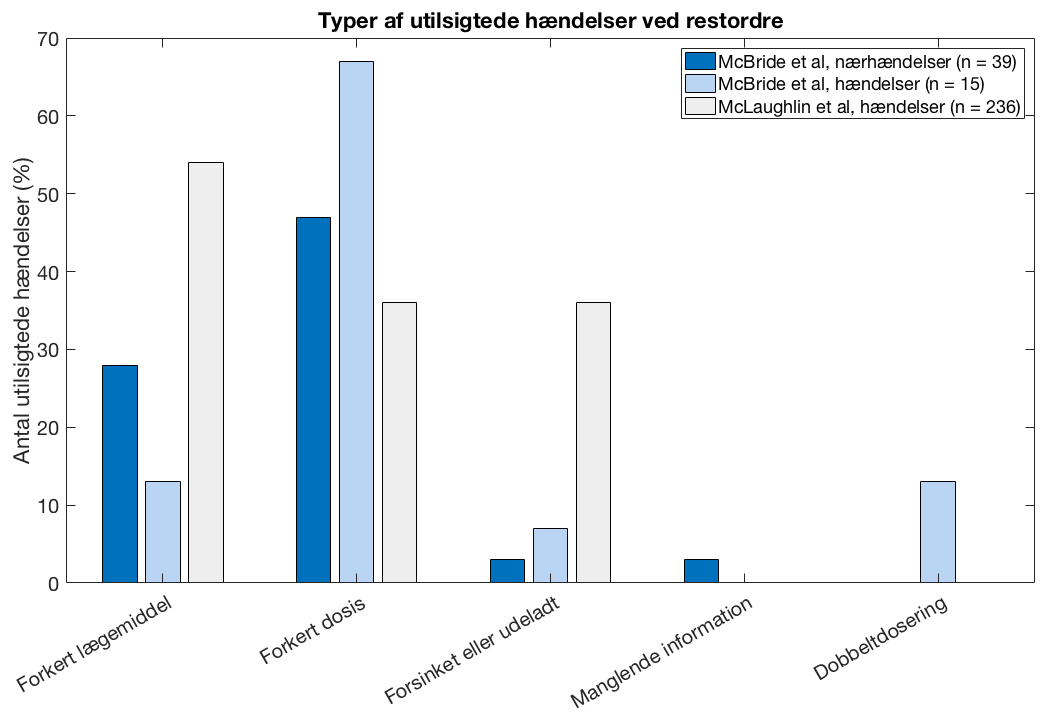
\includegraphics[width=1\textwidth]{billeder/UTH2.png} 
%	\caption{Utilsigtede hændelser opstået ved restordre~\citep{McLaughlin2013,McBride2013}.}
%	\label{fig:UTHrestordre}  
%\end{figure}
%
%Ud fra figur \ref{fig:UTHrestordre} fremgår det at forket dosis af lægemiddel og forsinket dosis var den hyppigste årsag til UTH'er ved restordre~\citep{McLaughlin2013,McBride2013}. Yderligere blev der i studierne identificeret UTH'er ved forsinket eller udeladt dispensering og administrering. Manglende information og dobbeltdosering blev påvist i et af studierne som en årsag til UTH'er ved restordre.~\citep{McLaughlin2013,McBride2013}
%
%
%
%%Lægemiddelskift medvirker til reportering af utilsigtede hændelser (UTH'er)~\citep{Amgros2015}.
%%Et præparatskift giver øgede administrative og kliniske udgifter og kan i værste fald betyde fejlmedicinering af patienter.
%%http://www.amgros.dk/media/1589/Amgros%20Årsmagasin.pdf
%
%%De hyppigste årsager til UTH'er på de danske hospitaler skyldes i år 2013 medicinering, hvilket udgjorde 23,97~\%.~\citep{Patientombuddet2013}. Antallet af rapporterede UTH'er i Region Nordjylland er steget med over 36\% fra år 2012 til 2014 ~\citep{Jensen2014}. Ud af 824 rapporterede UTH'er i år 2014 omhandlede 97\% af disse medicinering, 86\% administration af medicin og 41\% disponering~\citep{Jensen2014}. Det er i flere studier undersøgt de utilsigtede hændelser forårsaget af henholdsvis ordinationer, dispensering og administration af medicin, hvilket fremgår af tabel \ref{table:UTHordination}, \ref{table:UTHdispensering} og \ref{table:UTHAdministration}. En fælles årsag til de rapporterede UTH'er er forkert dosis, forkert lægemiddel og udeladelse af henholdsvis ordination, dispensering og administration.
%%
%%	\vspace{2mm}
%%\begin{longtable}{p{5cm}|p{4.2cm}|p{2cm}|p{2cm}}
%%	\caption{Utilsigtede hændelser ved ordinationer.}
%%	\vspace{2mm}
%%	\label{table:UTHordination} \\
%%\cellcolor[HTML]{C0C0C0} {\textbf{Årsager}} & 
%%{\cellcolor[HTML]{C0C0C0}\textbf{Sundhedsstyrelsen~\citep{Sundhedsstyrelsen2005}}} &
%%{\cellcolor[HTML]{C0C0C0}\textbf{Lisby et al~\citep{Lisby2005}}} &
%%{\cellcolor[HTML]{C0C0C0}\textbf{Tully et al~\citep{Tully2009}}} \\ \hline
%%%{\cellcolor[HTML]{C0C0C0}\textbf{4}} 
%%%\textbf{Metode} & Gennemgang af indberettede UTH'er & Observation, stikprøvekontrol, journalgennemgang & Gennemgang af medicinlister & Gennemgang af indberettede UTH'er \\ \hline
%%Forkert dosis & - & - & 12,5~\%  \\ \hline %& 29,6      \\ \hline
%%Forkert lægemiddel & 16,3~\% & - & - \\ \hline % & 14,5 \\ \hline
%%Forkert patient & 3,8~\% & - & - \\ \hline %& 11,2 \\ \hline
%%Intet lægemiddel ordineret & 20,7~\% & - & 15,9~\% \\ \hline % & 24,1 \\ \hline
%%Udeladelse af formulering & - & 38,0~\% & - \\ \hline %& - \\ \hline
%%Udeladelse af administrationsvej & - & 34,7~\% & - \\ \hline %& - \\ \hline
%%Udeladelse af doseringstidspunkt & - & 10~\% & 10,4*~\% \\ \hline %& - \\ \hline
%%Manglende angivelse af maskimal dosis & - & - & 12,1~\% \\ \hline %& -  \\ \hline
%%Overset kontraindikation & 14,3~\% & - & 0,3~\% \\ \hline %& 19,6 \\ \hline
%%\cellcolor[HTML]{C0C0C0} {\textbf{Total antal fejl}} & 
%%{\cellcolor[HTML]{C0C0C0}\textbf{526}} &
%%{\cellcolor[HTML]{C0C0C0}\textbf{320}} &
%%{\cellcolor[HTML]{C0C0C0}\textbf{3455}}
%%\end{longtable}
%%
%%Ud fra tabel \ref{table:UTHordination} fremgår det at de hyppigste årsager til UTH ved ordinationer skyldes 38~\% af de 320 rapportede UTH'er udeladelse af formulering og 34,7~\% administrationsvej~\citep{Lisby2005}. To studier påviste at i 20,7~\% ud af 526 og 15,9~\% af 3455 skyldes at intet lægemiddel var ordineret~\citep{Sundhedsstyrelsen2005, Tully2009}. Årsager som intet lægemiddel ordineret, udeladelse af doseringstidspunkt samt overset kontraindikation er dokumenteret af flere studier~\citep{Sundhedsstyrelsen2005, Lisby2005, Tully2009}. 
%%
%%\vspace{2mm}
%%\begin{longtable}{p{5cm}|p{4.2cm}|p{2cm}|p{2cm}}
%%	\caption{Utilsigtede hændelser ved dispensering.}
%%	\vspace{2mm}
%%	\label{table:UTHdispensering} \\
%%\cellcolor[HTML]{C0C0C0} {\textbf{Årsager}} & 
%%{\cellcolor[HTML]{C0C0C0}\textbf{Sundhedsstyrelsen~\citep{Sundhedsstyrelsen2005}}} &
%%{\cellcolor[HTML]{C0C0C0}\textbf{Lisby et al~\citep{Lisby2005}}} &
%%{\cellcolor[HTML]{C0C0C0}\textbf{Barker et al~\citep{Barker2002}}} \\ \hline
%%%\textbf{Metode} & Gennemgang af indberettede UTH'er & Observation, stikprøvekontrol, journalgennemgang & Gennemgang af medicinlister & Gennemgang af indberettede UTH'er \\ \hline
%%Forkert dosis & 26,6~\% & 29,4~\% &  20,0~\% \\ \hline
%%Forkert lægemiddel & 52,2~\% & - & - \\ \hline
%%Forkert tidspunkt & - & 1,1~\% & 40,3~\% \\ \hline
%%Udeladt dispensering & 11,4~\% & 41,2~\% & 27,9~\% \\ \hline
%%%Dispensering af et
%%Ikke ordineret lægemiddel & - & 29,4 & 4,8 \\ \hline
%%\cellcolor[HTML]{C0C0C0} {\textbf{Total antal fejl}} & 
%%{\cellcolor[HTML]{C0C0C0}\textbf{184}} &
%%{\cellcolor[HTML]{C0C0C0}\textbf{17}} &
%%{\cellcolor[HTML]{C0C0C0}\textbf{290}}
%%\end{longtable}
%%
%%Ud fra tabel \ref{table:UTHdispensering} fremgår det at de hyppigste årsager til UTH ved dispensering skyldes i 52,2~\% af de 184 rapporterede UTH'er forkert lægemiddel. Udover forkert lægemiddel blev der påvist forkert dosis, forkert tidspunkt eller udeladelse af dispensering samt ikke ordineret lægemiddel, hvor dette er dokumenteret i flere af studierne som værende en årsag til rapporteret UTH'er~\citep{Lisby2005, Sundhedsstyrelsen2005,Barker2002}.
%%
%%\vspace{2mm}
%%\begin{longtable}{p{5cm}|p{4.2cm}|p{2cm}|p{2cm}}
%%	\caption{Utilsigtede hændelser ved administration.}
%%	\vspace{2mm}
%%	\label{table:UTHAdministration} \\
%%\cellcolor[HTML]{C0C0C0} {\textbf{Årsager}} & 
%%{\cellcolor[HTML]{C0C0C0}\textbf{Sundhedsstyrelsen~\citep{Sundhedsstyrelsen2005}}} &
%%{\cellcolor[HTML]{C0C0C0}\textbf{Lisby et al~\citep{Lisby2005}}} &
%%{\cellcolor[HTML]{C0C0C0}\textbf{Barker et al~\citep{Barker2002}}} \\ \hline
%%%\textbf{Metode} & Gennemgang af indberettede UTH'er & Observation, stikprøvekontrol, journalgennemgang & Gennemgang af medicinlister & Gennemgang af indberettede UTH'er \\ \hline
%%Forkert dosis & 37,5~\% & - & 20,0~\% \\ \hline
%%Forkert lægemiddel & 19,1~\% & - & - \\ \hline
%%Forkert tidspunkt & 8,9~\% & - & 40,3~\% \\ \hline
%%Forkert patient & - & 15,7~\% &  - \\ \hline
%%Udeladt administration & 15,0~\% & - & 27,9~\% \\ \hline
%%Manglende identifikation af patient & - & 78,9~\% & - \\ \hline
%%\cellcolor[HTML]{C0C0C0} {\textbf{Total antal fejl}} & 
%%{\cellcolor[HTML]{C0C0C0}\textbf{839}} &
%%{\cellcolor[HTML]{C0C0C0}\textbf{190}} &
%%{\cellcolor[HTML]{C0C0C0}\textbf{290}}
%%\end{longtable}
%%\vspace{0.25cm}
%%
%%Ud fra tabel \ref{table:UTHAdministration} fremgår det at de hyppigste årsager til UTH ved administration i 78,9~\% af de 190 rapporterede UTH'er manglende patientidentifikation~\citep{Lisby2005}. I et af studierne skyldes 40,3~\% ud af 290 af tilfældene forkert tidspunkt~\citep{Barker2002} og i 37,5~\% af 839 forkert dosis~\citep{Sundhedsstyrelsen2005}. Forket dosis, forkert tidspunkt og udeladt administration var dokumenteret i flere studier~\citep{Lisby2005,Sundhedsstyrelsen2005,Barker2002}.
%
